\documentclass{article}

\usepackage{amsfonts}
\usepackage{graphicx}
\usepackage{amssymb}
\usepackage{amsmath}
\usepackage{listings}


\DeclareMathOperator{\sech}{sech}
\newcommand{\NN}{\mathbb{N}}
\newcommand{\RR}{\mathbb{R}}
\newcommand{\QQ}{\mathbb{Q}}
\newcommand{\ZZ}{\mathbb{Z}}
\newcommand{\dV}{\;\mathrm{d}V}
\newcommand{\dA}{\;\mathrm{d}A}
\newcommand{\dx}{\;\mathrm{d}x}
\newcommand{\dy}{\;\mathrm{d}y}
\newcommand{\dz}{\;\mathrm{d}z}
\newcommand{\cA}{\mathcal{A}}
\newcommand{\Bb}{\mathcal{B}}
\newcommand{\Ww}{\mathcal{W}}
\newcommand{\Dd}{\mathcal{D}}
\newcommand{\Ss}{\mathcal{S}}
\newcommand{\Ee}{\mathcal{E}}
\DeclareMathOperator{\im}{im}


\setlength\parindent{18pt}

\begin{document}

Textbook Section 6.1:

2) The critical point of the given autonomous system is $(1, 1)$.
J = $\begin{bmatrix}
    1 & -1 \\
    1 & 3
\end{bmatrix}$.
The Jacobian matrix has a repeated eigenvalue of $2$.
Since the eigenvalue is positive and real, the critical point $(1, 1)$
is an unstable node. It matches Figure 6.1.16.

4) The critical point of the given autonomous system is $(1, -1)$.
J = $\begin{bmatrix}
    2 & -2 \\
    1 & 4
\end{bmatrix}$.
The Jacobian matrix has complex eigenvalues of $3 \pm i$.
Since the real parts of the eigenvalues are positive, the critical point
$(1, -1)$ is an unstable focus (or spiral). It matches 6.1.13.

6) The given autonomous system has two critical points at $(-2, \frac{2}{3})$
and $(2, -\frac{2}{5})$.
J = $\begin{bmatrix}
    -4 & -15 \\
    -2x & 0
\end{bmatrix}$.

For the critical point $(-2, \frac{2}{3})$, the eigenvalues
are $-2 \pm 2 \sqrt{14} i$.
These are complex numbers with negative real parts, indicating that
this critical point is a stable focus (or spiral).

For the critical point $(2, -\frac{2}{5})$, the eigenvalues are
$6$ and $-10$. These are real numbers of opposite signs, indicating that
this critical point is a saddle point.

This system matches 6.1.18.

Textbook Section 6.2:

2) For the linear system given by $\frac{dx}{dt} = 4x - y$ and
$\frac{dy}{dt} = 2x + y$, the eigenvalues of the coefficient matrix are
$3$ and $2$.

In this case, both eigenvalues are positive real numbers. Therefore, the
critical point (0, 0) is unstable.

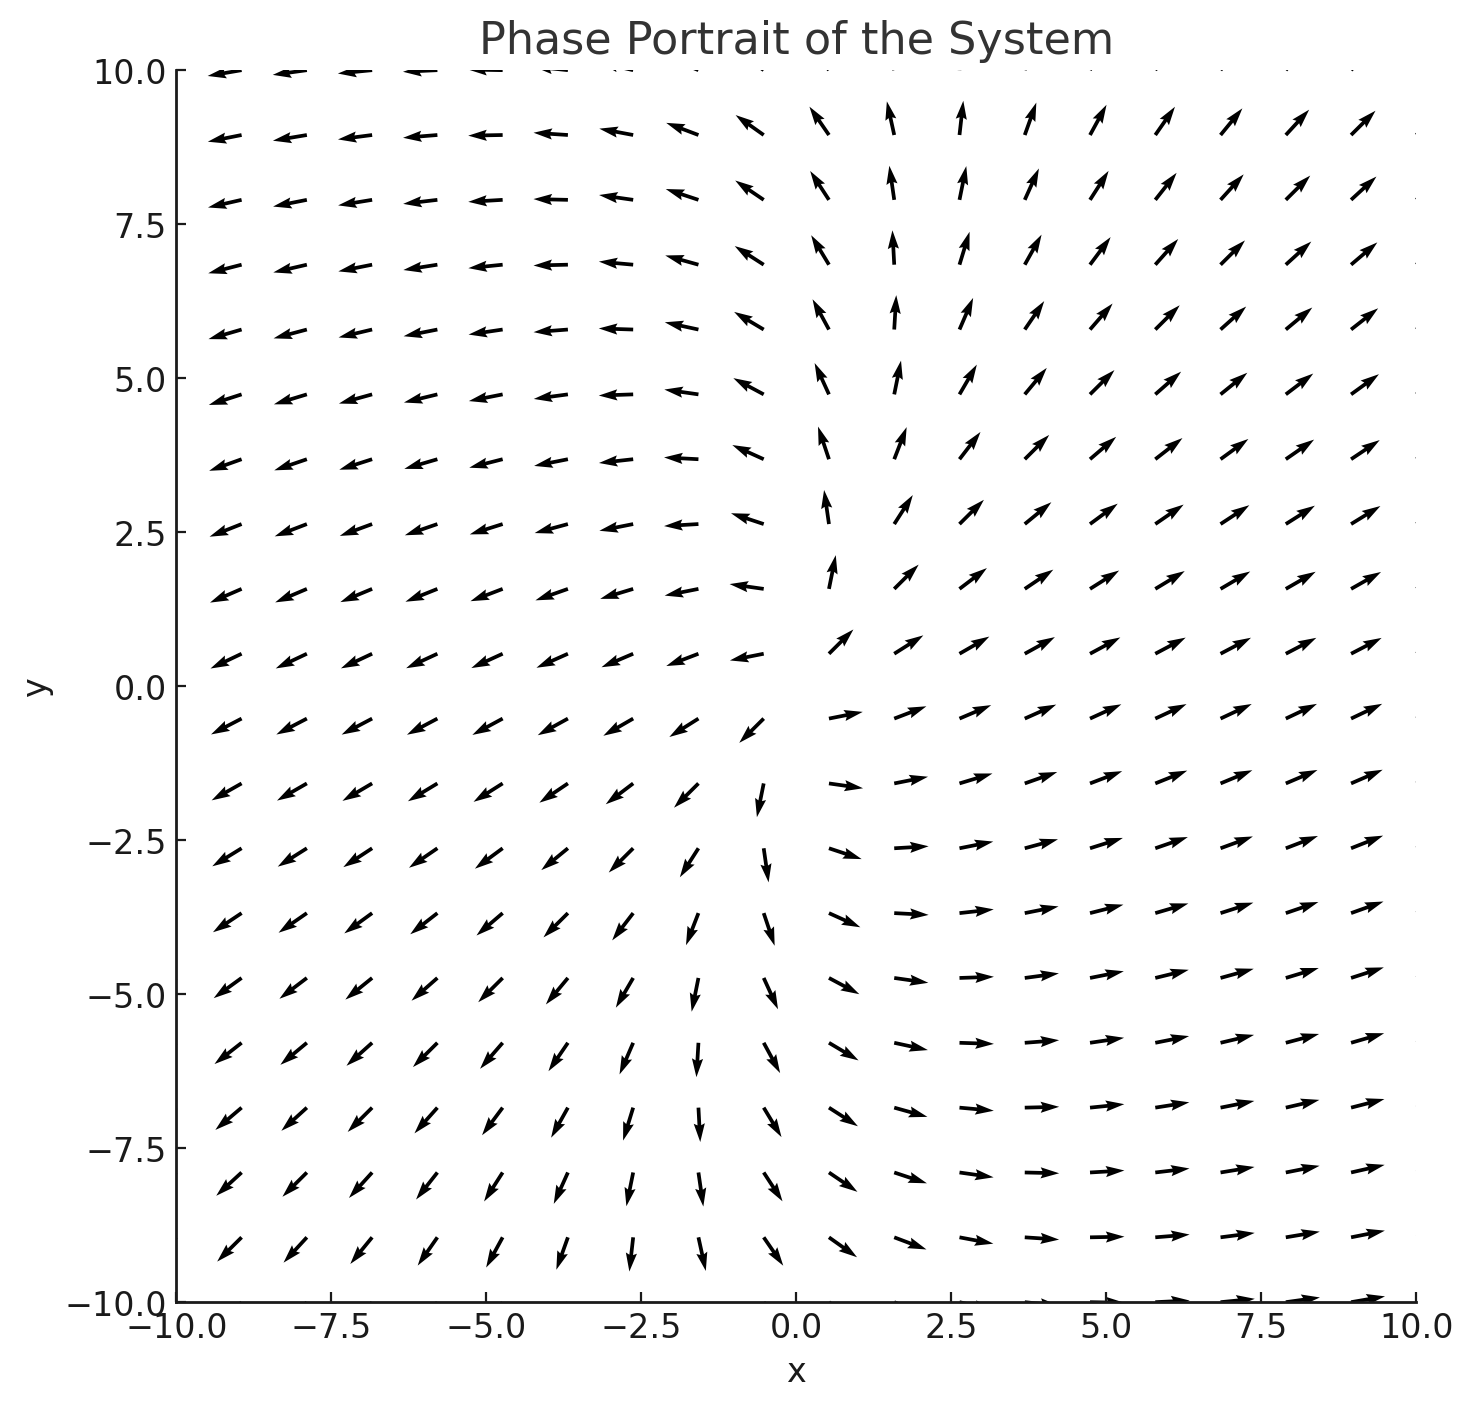
\includegraphics[width=\linewidth]{6_2_2}

8) For the linear system given by $\frac{dx}{dt} = x - 3y$ and
$\frac{dy}{dt} = 6x - 5y$, the eigenvalues of the coefficient matrix are
$-2 \pm 3i$.

In this case, both eigenvalues have negative real parts and non-zero imaginary parts.
Therefore, the critical point (0, 0) is asymptotically stable.

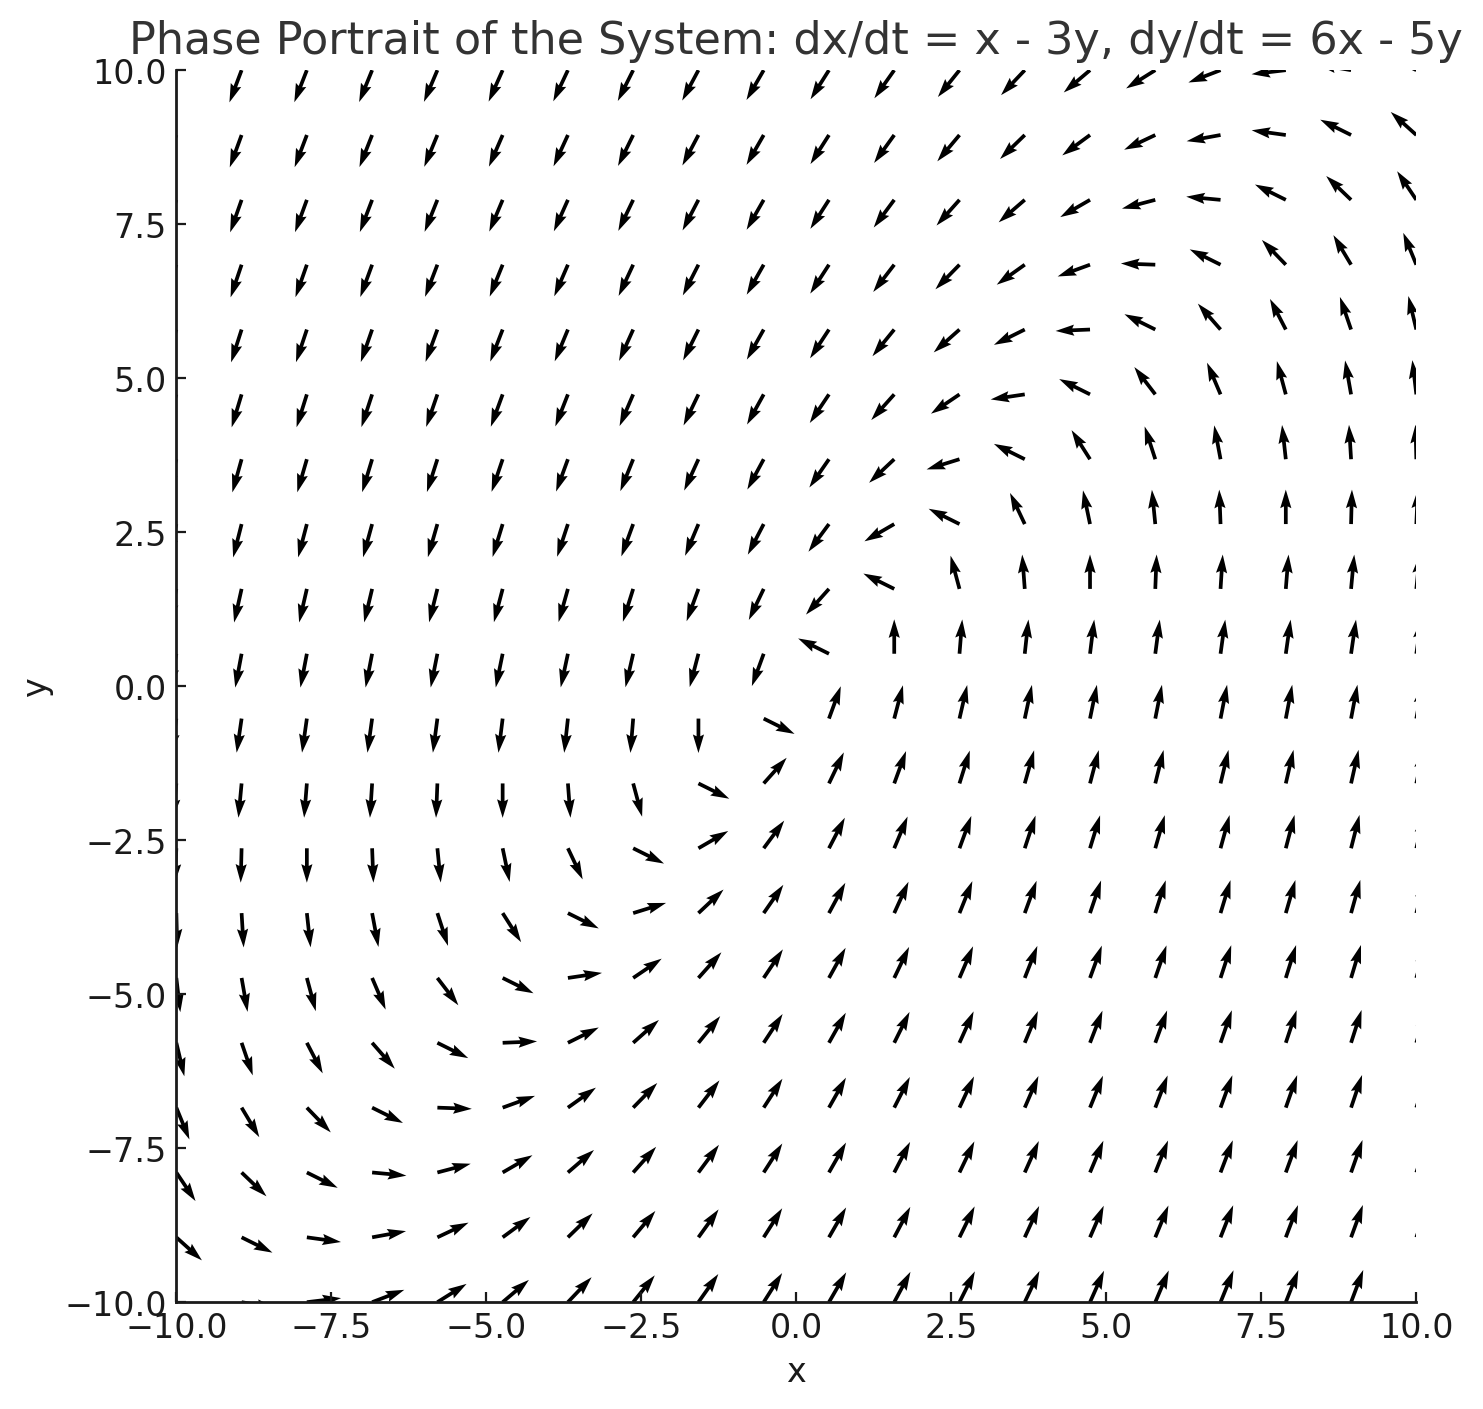
\includegraphics[width=\linewidth]{6_2_8}

14) For the given system $\frac{dx}{dt} = x + y - 7$ and
$\frac{dy}{dt} = 3x - y - 5$, the eigenvalues of the coefficient matrix are
$-2$ and $2$.

In this case, the eigenvalues are real and unequal. Hence the critical point
is of the same type and stability as the associated linear system. Since one
of the eigenvalues is positive, the critical point is unstable.

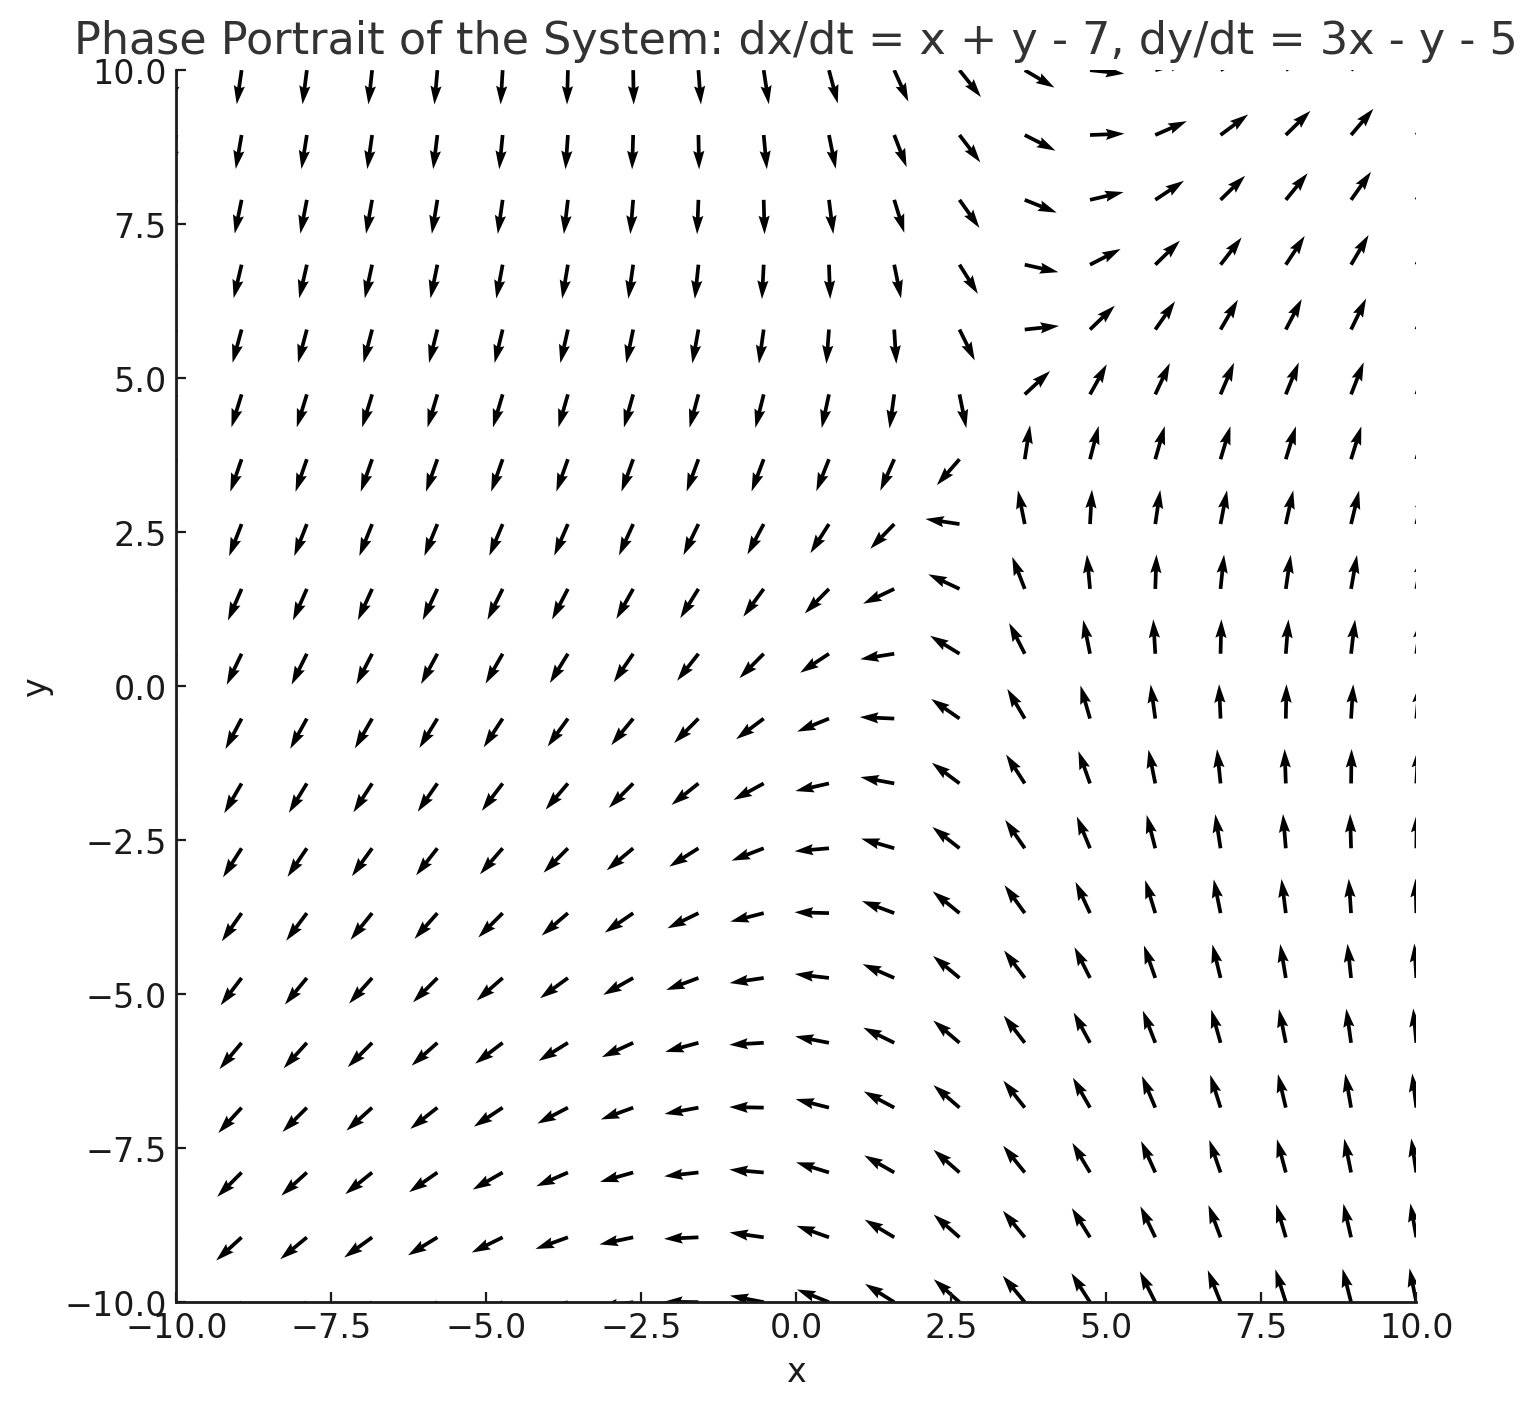
\includegraphics[width=\linewidth]{6_2_14}

30) The system $\frac{dx}{dt} = y - 1$ and $\frac{dy}{dt} = x^2 - y$
has two critical points at $(-1, 1)$ and $(1, 1)$.

J = $\begin{bmatrix}
    0 & 1 \\
    2x & -1
\end{bmatrix}$.

For the critical point $(-1, 1)$, the eigenvalues
are $-\frac{1}{2} \pm \frac{\sqrt{7}}{2} i$.
These are complex numbers with negative real parts, indicating that
this critical point is a stable focus (or spiral).

For the critical point $(1, 1)$, the eigenvalues are
$1$ and $-2$. These are real numbers of opposite signs, indicating that
this critical point is a saddle point.

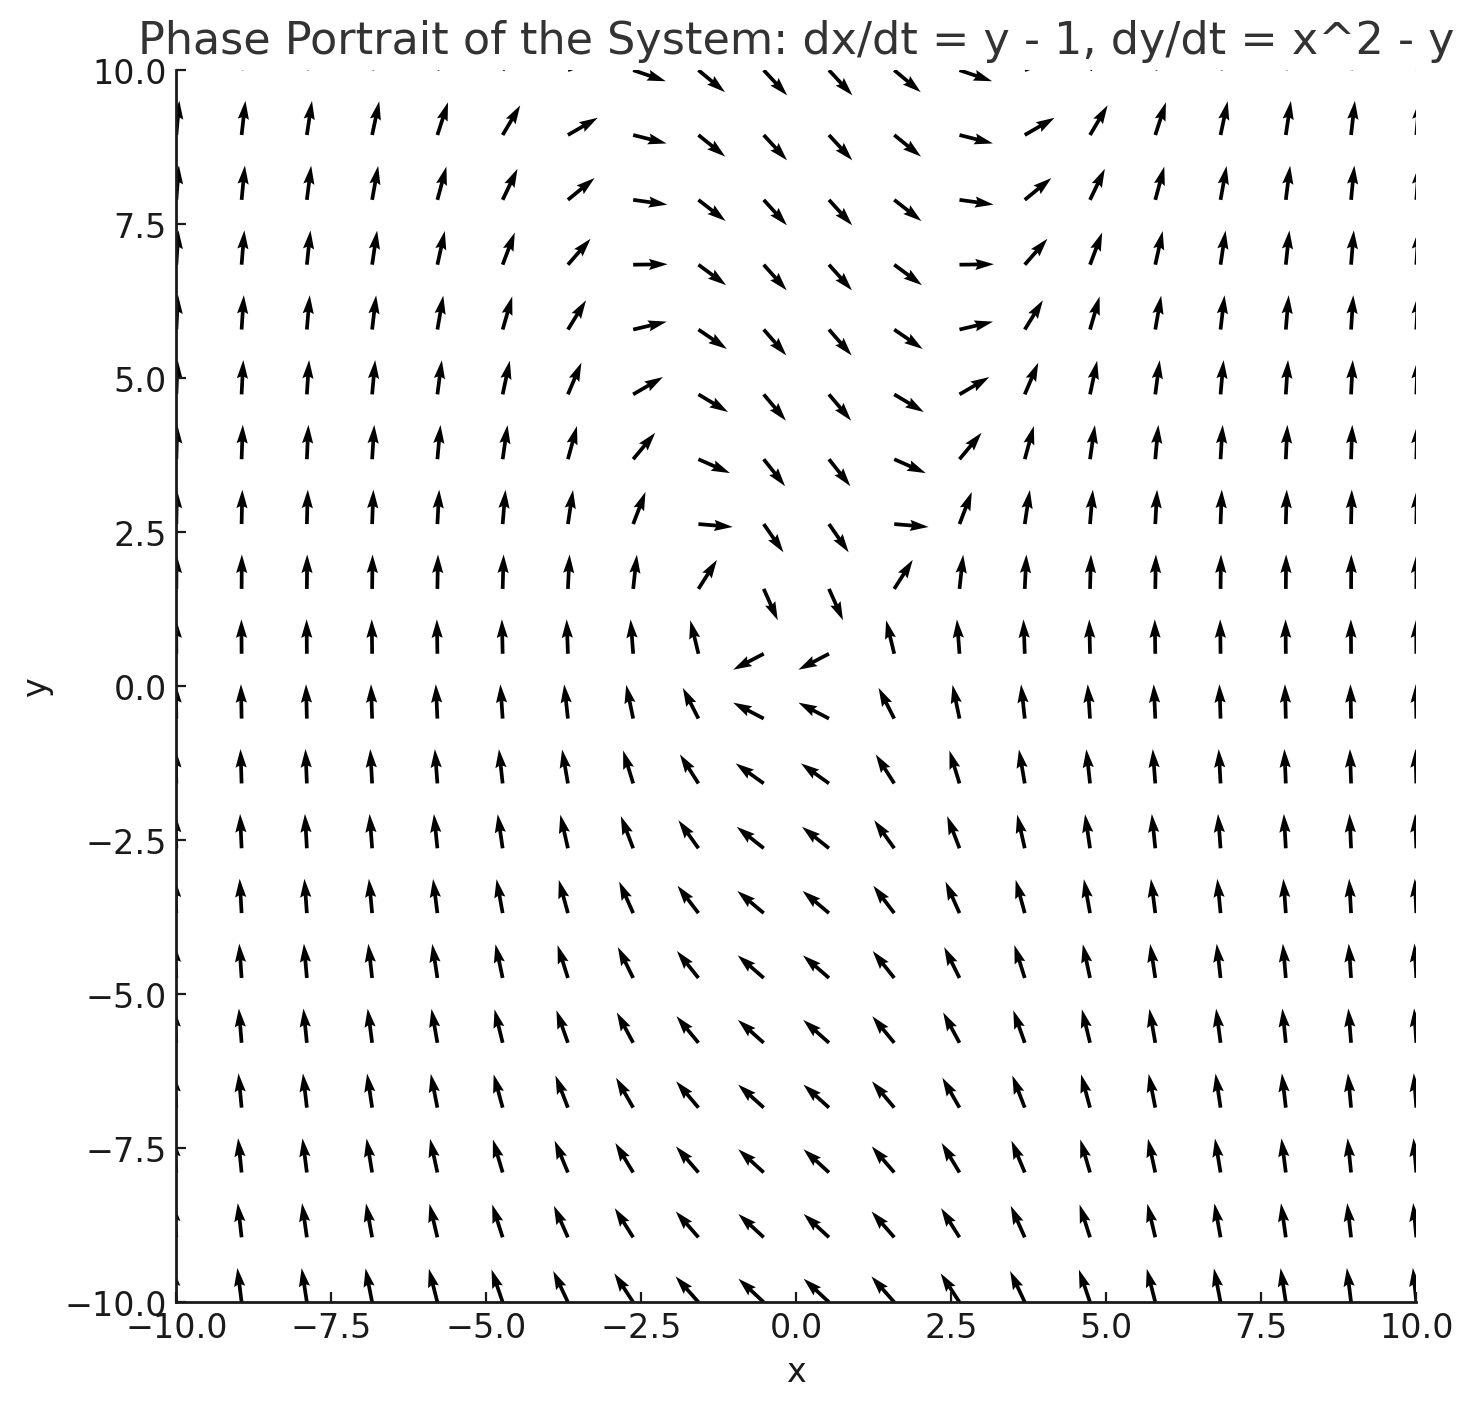
\includegraphics[width=\linewidth]{6_2_30}

Textbook Section 6.3:

1) The Jacobian matrices at the critical points $(0, 0)$ and
$(75, 50)$ for the given predator-prey system are as follows:

At $(0, 0)$:
J = $\begin{bmatrix}
    200 & 0 \\
    0 & -150
\end{bmatrix}$.

At $(75, 50)$:
J = $\begin{bmatrix}
    0 & -300 \\
    100 & 0
\end{bmatrix}$.

For the critical point $(0, 0)$, the Jacobian matrix is diagonal
with eigenvalues $200$ and $-150$. These are real numbers of opposite
signs, indicating that the critical point is a saddle point and thus
unstable.

For the critical point $(75, 50)$, the Jacobian matrix has off-diagonal
elements with a zero trace. The eigenvalues of the matrix will be purely
imaginary, indicating that the critical point is a center.

2) Given the quotient system $\frac{dy}{dx} = \frac{-150y + 2xy}{200x - 4xy}$,
this can be simplified to
$\frac{dy}{dx} = \frac{y(-150 + 2x)}{x(200 - 4y)}$.

This becomes $\frac{200 - 4y}{y} dy = \frac{150 - 2x}{x} dx$.

Integrating both sides gives
$\int \frac{200 - 4y}{y} dy = \int \frac{150 - 2x}{x} dx$.

This gives:
$200 \ln(y) - 4y = 150 \ln(x) - 2x + C$.

Rearranging this gives:
$200 ln(y) + 150 ln(x) - 2x - 4y = C$
as expected.

The values of the constant C for the contour curves passing through
the given points are as follows:

At $(75, 100)$, $C = -550 + 150 \ln(75) + 200 \ln(100)$

At $(75, 150)$, $C = -750 + 150 \ln(75) + 200 \ln(150)$

At $(75, 200)$, $C = -950 + 150 \ln(75) + 200 \ln(200)$

At $(75, 250)$, $C = -1150 + 150 \ln(75) + 200 \ln(250)$

At $(75, 300)$, $C = -1350 + 150 \ln(75) + 200 \ln(300)$

\end{document}
